The goals for this thesis where twofold. Firstly, the applicability of numerous machine learning approaches for activity prediction, and
secondly the application of feature engineering methods to the base datasets.
\\\\
The first goal was addressed by implementing \textit{k nearest neighbor}, \textit{random forest} and \textit{neural network} algorithms.
The results from those baseline implementations are very promising. The second goal builds upon the first goal. Through the implementation of various feature engineering 
methods the results of the baseline machine learning algorithms improved for a select number of configurations. An especially noteworthy feature engineering method in this context is
\acrshort*[]{smote}. Through the balancing of the provided datasets using \acrshort*[]{smote} the accuracy of all models improved.
When comparing the different machine learning approaches the \textit{random forest} algorithm was able to achieve the best performance overall.

The overall performance of the models compares well to the scoring functions introduced in \cite[]{Birklbauer2021}.
The following table represents the results for the \acrshort*[]{ache} protein in \cite[]{Birklbauer2021}:
\begin{figure}[H]
    \begin{center}
        \caption[]{Scoring results for ACHE Birklbauer}
        \label{fig:ache_birklbauer}
        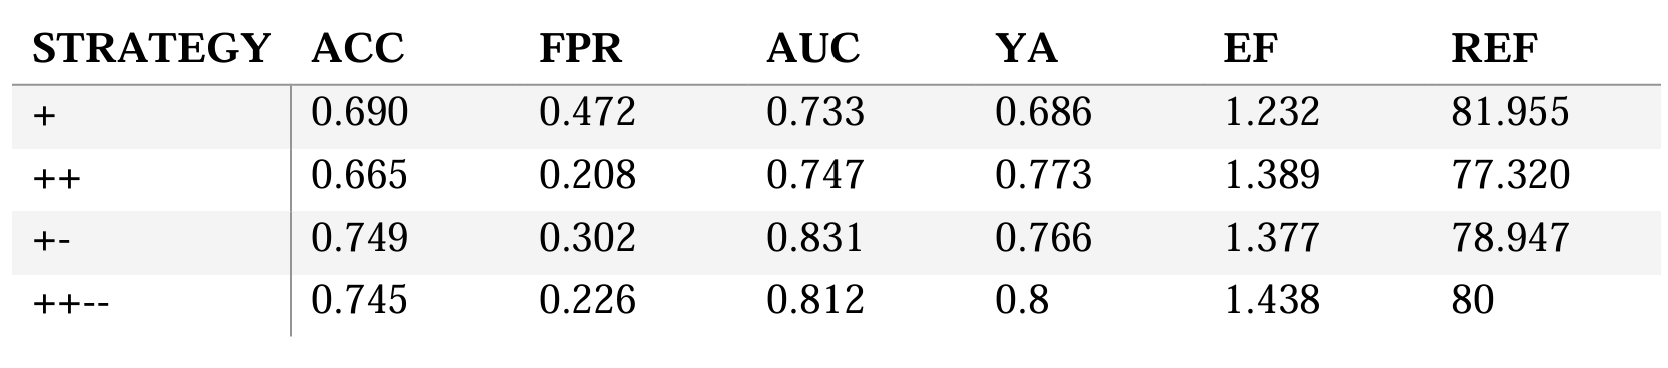
\includegraphics[width=14cm]{discussion/Birklbauer_ACHE.png}
    \end{center}
\end{figure}
The following results were achieved for the \acrshort*[]{ache} protein using the methods proposed in this thesis:
\begin{table}[H]
    \begin{center}
        \caption{Acetylcholinesterase performance test-set}
        \begin{tabular}{lrrrrrr}
            \toprule
            Name             & ACC    & FPR    & AUC    & YA     & EF     & REF     \\
            \midrule
            baseline\_rf     & 0.8106 & 0.3285 & 0.7992 & 0.7716 & 1.4161 & 92.6829 \\
            fe\_smote\_rf    & 0.8007 & 0.3358 & 0.7894 & 0.7653 & 1.4046 & 91.4634 \\
            fe\_smote\_nn    & 0.7708 & 0.2993 & 0.7650 & 0.7684 & 1.4102 & 82.9268 \\
            baseline\_nn     & 0.7674 & 0.2920 & 0.7626 & 0.7701 & 1.4134 & 81.7073 \\
            fe\_rf\_per\_knn & 0.7575 & 0.4307 & 0.7420 & 0.7177 & 1.3172 & 91.4634 \\
            baseline\_knn    & 0.6844 & 0.5766 & 0.6629 & 0.6520 & 1.1966 & 90.2439 \\
            fe\_rf\_mdi\_knn & 0.5515 & 0.4307 & 0.5530 & 0.5986 & 1.0987 & 59.8639 \\
            \bottomrule
        \end{tabular}
    \end{center}
\end{table}

The comparison between the two tables underlines the performance improvements of the machine learning approaches
over the simple scoring functions introduced in \cite[]{Birklbauer2021}.
Generally the improvements in \acrshort*[]{acc} and \acrshort*[]{ref} are most notable.
The improvements in the \acrshort*[]{ref} metric are of particular interest, as there is less money spent on investigating false positive compounds.
Similar performance benefits can be observed for the other protein complexes.